% !TEX encoding = UTF-8 Unicode
%!TEX root = ../Main/thesis.tex
% !TEX spellcheck = en-US
%%=========================================
\documentclass[../Main/thesis.tex]{subfiles}
\begin{document}
	\chapter[Conclusions]{Conclusion}
	\label{sec:conclusions}
	 In section \ref{sec:comp}, the results obtained from the high frequency resonance technique and the scheme presented in this thesis are compared.
	 Section \ref{sec:summary_and_conclusions} presents a summary, followed by a discussion regarding the main results, and recommendations.

	
	%%=========================================
	\section{Comparison of results}
		\label{sec:comp}
	Figure \ref{fig:hfrt-method} and \ref{fig:yapi-method} show the frequency spectrum obtained from the high frequency resonance technique (HFRT), and the method proposed in this thesis, respectively. The magnitude of each peak in the spectrum given by the HFRT is in G or $mm/s^{2}$. Whereas, the magnitude of the peaks obtain in this thesis are in energy square per Hertz. That is, the energy contribution per Hertz. Regardless, for bearing fault detection, a high magnitude defect frequency, corresponds to a severe bearing fault. The HFRT and the method presented in this thesis, can both identify the inner race defect frequency.
	\justify
	 Both Figures represent the spectrum of a signal obtained from a bearing with an inner ring defect. The latter can produce a noisy frequency spectrum when the HFRT is applied. This can been seen from Figure \ref{fig:hfrt-method}, which shows a relatively noisy frequency spectrum. The peaks are so closed to one an other that, it can be tedious to clearly identify a specific peak.
	Although the HFRT applies a series of filtering in order to strip out irrelevant signal components, the resulting frequency spectrum still contains  peaks embedded in noise. Consequently, identifying bearing faults with certainty, can be challenging. 
	
	\begin{figure}[H]
		\centering
		%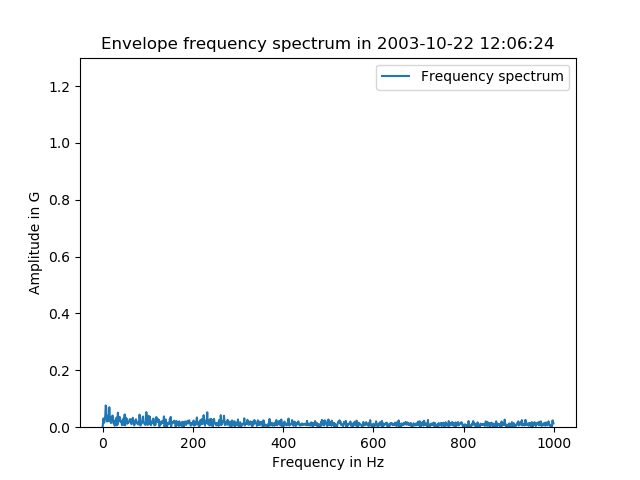
\includegraphics[width=0.7\linewidth]{../fig/bpfi/first_day_spectrum}
		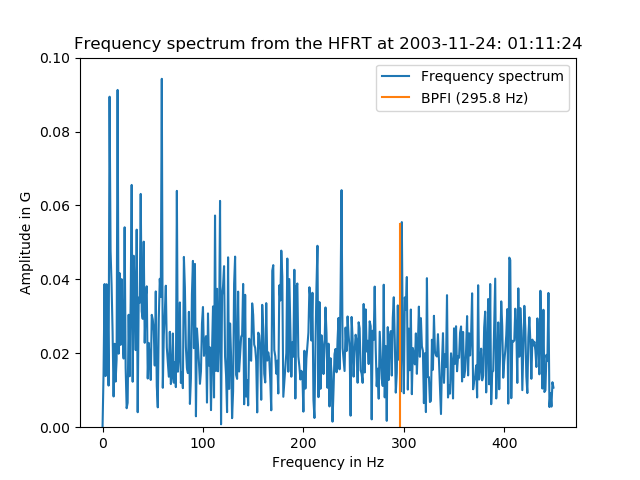
\includegraphics[width=0.7\linewidth]{../fig/hfrt}
		\caption{Frequency spectrum with an identified ball pass inner race defect frequency obtained from the high frequency resonance technique (HFRT).}
		\label{fig:hfrt-method}
		
		\begin{figure}[H]
			\centering
			%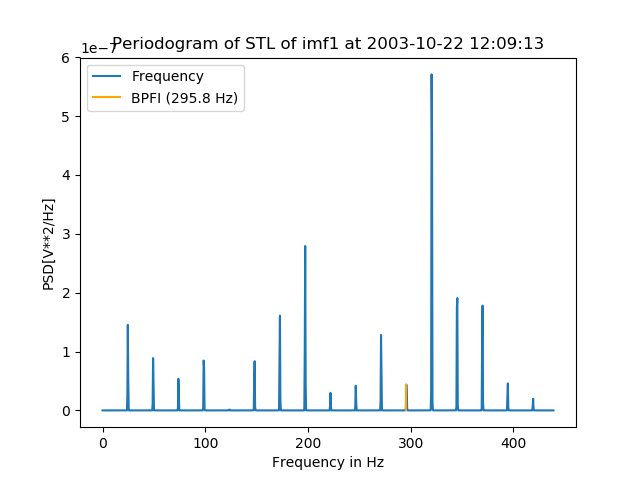
\includegraphics[width=0.8\linewidth]{../fig/periodogram_bpfi/start_imf1_bpfi}
			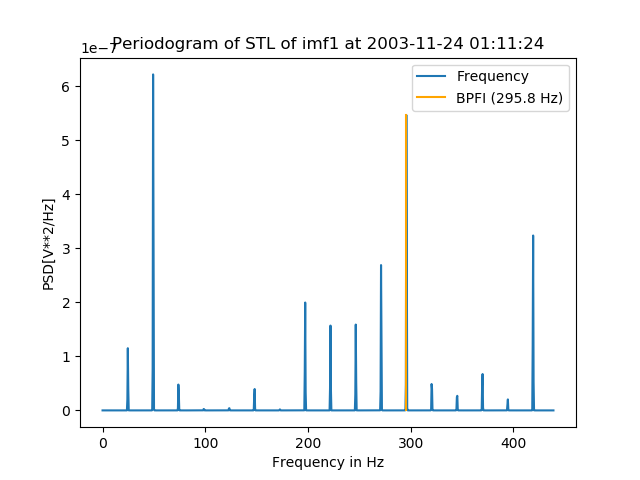
\includegraphics[width=0.7\linewidth]{../fig/periodogram_bpfi/end_imf1_bpfi}
			\caption{Frequency spectrum with an identified ball pass inner race defect frequency obtained from the method posited in this thesis.}
			\label{fig:yapi-method}
		\end{figure}
	\end{figure}
\justify
In contrast, Figure \ref{fig:yapi-method} shows a clear spectrum with conspicuous frequency peaks. By applying the empirical mode decomposition on the target vibration signal, the most relevant information is extracted. Furthermore, the seasonal component of the extracted intrinsic mode function represents a relatively noiseless signal. This means that only part of the signal containing diagnostic information are captured. With enough information of the machine, the origin of most peaks on the frequency spectrum could be (almost) explained. 
This make bearing fault diagnosis easier and accurate, as we are only restricted to few frequency peaks to analyze.

	\section{Summary}
	\label{sec:summary_and_conclusions}
	 The proclivity of machines towards failure, imposes a monitoring and maintenance scheme, in order to avoid unexpected and catastrophic breakdown. To mitigate such events, most machines are equipped with an array of sensors, collecting continuously data. A myriad of methods and algorithms make it possible to analyze the data generated, in order to detect as early as possible any sign of failure, and take necessary actions.
	\justify
	By facilitating rotational movements, bearings are critical part of nearly all rotating equipment. Being continually subjected to extensive load, bearing failures represent more than 40$\%$ of defect in rotating machines. In most industries, Fourier transform is the pillar of bearing fault detection, and is a corner stone of nearly all methods.
	One of the most widely used scheme is the so called high frequency resonance technique. 
	In the latter, a bearing vibration signal is filtered to remove noise, and isolate desirable components, before subsequently being decomposed into a spectrum of frequencies. For a bearing, the failure frequency is derived from its geometrical components and the rotational speed of the machine on which it is mounted. Once the failure frequencies are available (given by the manufacturer), it suffices to search for them in the frequency spectrum, derived from the Fourier transform. 
	\justify
	The high frequency resonance technique although widely used, can produce a very noisy spectrum, in particular when the bearing is subjected to a sever inner race defect. This can render fault detection very challenging. In this thesis therefore, a new method is presented to mitigate this issue.
	This new scheme consists of decomposing an input bearing vibration signal into successive high to low frequency components called intrinsic mode functions (IMFs). This is achieved through the so called empirical mode decomposition (EMD). The latter is part of the Hilbert-Huang transform, which couples the EMD with the Hilbert transform, in order to derive well define instantaneous frequencies and amplitude. The former and the latter are very important in frequency and amplitude modulated problems.
	\justify
	Once the intrinsic mode functions (IMFs) have been computed, the first IMF is selected. Furthermore, its seasonal trend is computed through the seasonal trend decomposition method by LOESS (STL). The STL is a computational efficient method that decomposes a signal into its trend and seasonal parts. The trend is a monotone function, while the seasonal part is a periodic oscillatory sinusoidal. Furthermore, the power spectrum density of the seasonal component of the first intrinsic mode function is approximated. This is achieved through the periodogram method (approximation of the power spectral density). The result is a frequency spectrum, with clear and conspicuous peaks.
	\justify
	To test the efficiency of the proposed new method, a case study was performed with bearings vibration data, obtained from an experiment run by the diagnosis branch of the national aeronautical administration (NASA). The application of the new scheme resulted in a conspicuous energy distribution per frequency contribution, where bearing failure frequencies are clearly identifiable. In addition, bearing failure characteristics such harmonics, and the rotation speed of the motor housing the bearings, are all visible in the estimated spectrum.
	\justify
	The Hilbert-Huang transform, through the empirical mode decomposition (EMD), boasts itself in generated mono components intrinsic mode functions. However, the EMD suffers from what is known as mode mixing, which makes an IMF not exactly mono component. This is precisely the reason why in this thesis, the seasonal component of each IMF is extracted in order to circumvent the mode mixing issue.
	\justify
	The result obtained are satisfactory in the sens that, bearing failure frequencies are clearly identified. However, only two types of bearing failure were tested in this thesis: namely fault occurring in the inner and outer ring. The justification is that these are the prevalent faults encountered. As an extension to this work, the new method could be applied to detecting the whole range of bearing failure, in order to further corroborate its full validity. In addition, since the data for this case study was obtained under a control experiment, the new scheme could be applied to data from real industrial processes to broadly justify its validity.

	
\end{document}
